\newpage
\section{Teksturowanie}
Teksturowanie polega na nałożeniu na powierzchnię obiektu mapy bitowej. Mapa ta, by być właściwie nałożona na obiekt, musi być odpowiednio na nim odwzorowana. OpenGL pozwana na określić odwzorowanie punktu trójkąta na punkt tekstury. Tekstura ładowana jest w postaci kwadratowej mapy bitowej o wielkości będącej potęgą liczby 2. W programie zastosowano tekstury z rastrowych plików graficznych w formacie \textit{TARGA} (.tga). 
Korzystanie z tekstur wymagało skonfigurowani odpowiednich parametrów oraz wywołania metody \lstinline{glEnable} z parametrem w odpowiednim widoku (listing \ref{lst:texturee}). Zastosowano opcję \textit{Cull Face}, która odpowiada za teksturowanie tylko jednej strony powierzchni, co redukuje obliczenia. W przypadku rysowania trójkątów stronę powierzchni określa kolejność rysowania wierzchołków.

\begin{lstlisting}[language=C++, caption=Konfiguracja ustawień teksturowania., label={lst:texturee}]
glTexParameteri(GL_TEXTURE_2D, GL_TEXTURE_MAG_FILTER, GL_LINEAR);
glTexEnvi(GL_TEXTURE_ENV, GL_TEXTURE_ENV_MODE, GL_MODULATE);
...
glEnable(GL_TEXTURE_2D);
glEnable(GL_CULL_FACE);
\end{lstlisting}

\subsection{Klasa tekstury}
W celu zarządzania teksturami utworzona została klasa \lstinline{Texture}, która odpowiedzialna jest za wczytywanie, przetrzymywanie danych i wkładanie tekstury do bufora biblioteki OpenGL. Klasa ta przechowuje tablicę bajtów z danymi tekstury, jej wysokość i szerokość oraz format danych.
Przed narysowaniem danego modelu tekstura jest wkładana do bufora, za co odpowiedzialna jest metoda \lstinline{apply} pokazana na listingu \ref{lst:texture-apply}.
\clearpage
\begin{lstlisting}[language=C++, caption=Definicja klasy \lstinline{Texture}., label={lst:texture}]
class Texture
{
public:
    Texture(std::string filename);
    ~Texture();
    void apply();
private:
    GLbyte *pBytes;
    GLint width = 0;
    GLint height = 0;
    GLint components = GL_RGB8;
    GLenum format = GL_BGR_EXT;
};
\end{lstlisting}


\begin{lstlisting}[language=C++, caption=Metoda \lstinline{apply} klasy \lstinline{Texture}., label={lst:texture-apply}]
void Texture::apply()
{
    glTexImage2D(GL_TEXTURE_2D, 0, components, width, height, 0, format, GL_UNSIGNED_BYTE, pBytes);
}
\end{lstlisting}

\subsection{Klasa Point i model czworościanu}
By dodać możliwości teksturowania do obecnych modeli, modyfikacji uległa klasa \lstinline{Point}, do której zostały dodane współrzędne \textit{tx} i \textit{ty} określające odwzorowanie punktu w układzie współrzędnych tekstury. Wartości tych parametrów są liczbami z przedziału $<0;1>$. Punkt ten przekazywany jest do biblioteki OpenGL w metodzie rysującej \lstinline{drawWithColor}. Wywołanie odpowiedniej metody widoczne jest w linijce 5 listingu \ref{lst:point-dwc}.
\begin{lstlisting}[language=C++, caption=Konstruktor klasy \lstinline{Point}., label={lst:point-construct}]
Point(float x, float y, float z, GLubyte r, GLubyte g, GLubyte b, float tx = 0, float ty = 0)
        : color({r, g, b}), x(x), y(y), z(z), tx(tx), ty(ty){};

\end{lstlisting}
\begin{lstlisting}[language=C++, caption=Metoda \lstinline{drawWithColor} klasy \lstinline{Point}., label={lst:point-dwc}]
void Point::drawWithColor()
{
    color.apply();
    glNormal3f(nx, ny, nz);
    glTexCoord2f(tx, ty);
    glVertex3f(x, y, z);
}
\end{lstlisting}

Z tak zmodyfikowaną klasą \lstinline{Point} można było zdefiniować model \lstinline{TexModel}, którego konstruktor klasy tworzył punkty w odpowiedniej kolejności (listing \ref{lst:texmodel-con}), a metoda \lstinline{renderTriangles} rysowała je na ekranie (listing \ref{lst:texmodel-render}). 
\begin{lstlisting}[language=C++, caption=Konstruktor klasy \lstinline{TexModel}., label={lst:texmodel-con}]
TexModel::TexModel()
{
    points.push_back(std::vector<Point>({
        Point(1., 1., 0., 255, 255, 255, 1, 0),
        Point(5., 1., 0., 255, 255, 255, 0, 0),
        Point(3., 5., 0., 255, 255, 255, 0.5, 1)}));
    points.push_back(std::vector<Point>({
        Point(1., 1., 0., 255, 255, 255, 1, 0),
        Point(3., 2.5, 4., 255, 255, 255, 0.5, 1),
        Point(5., 1., 0., 255, 255, 255, 0, 0)}));
    points.push_back(std::vector<Point>({
        Point(3., 5., 0., 255, 255, 255, 1, 0),
        Point(5., 1., 0., 255, 255, 255, 0, 0),
        Point(3., 2.5, 4, 255, 255, 255, 0.5, 1)}));
    points.push_back(std::vector<Point>({
        Point(3., 2.5, 4, 255, 255, 255, 0.5, 1),
        Point(1., 1., 0., 255, 255, 255, 1, 0),
        Point(3., 5., 0., 255, 255, 255, 0, 0)}));
}
\end{lstlisting}
\clearpage
\begin{lstlisting}[language=C++, caption=Metoda \lstinline{renderTriangles} klasy \lstinline{TexModel}., label={lst:texmodel-render}]
void TexModel::renderTriangles()
{
    glBegin(GL_TRIANGLES);
    for (auto &&triangle : points)
    {
        for (auto &&point : triangle)
        {
            point.drawWithColor();
        }
    }
    glEnd();
}
\end{lstlisting}

\subsection{Wyświetlanie czworościanu i modelu jajka z teksturą}

W celu prezentacji wyświetlania modeli z teksturą utworzony został widok \lstinline{TexModelView}, gdzie w metodzie \lstinline{render} wyświetlane są dwa obracające się czworościany, na które zostały nałożony tekstury. Zostały one utworzone jako obiekty przechowywane w zmiennych klasy widoku.
\begin{lstlisting}[language=C++, caption=Zmienne klasy \lstinline{TexModelView} odpowiedzialne za model i tekstury., label={lst:texmodelview-hpp}]
TexModel texModel;
Texture texture1 = Texture("src/textures/paput.tga");
Texture texture2 = Texture("src/textures/D5_t.tga");
\end{lstlisting}

\begin{lstlisting}[language=C++, caption=Metoda \lstinline{render} klasy \lstinline{TexModelView}., label={lst:texmodelview-render}]
void TexModelView::render()
{
    glLoadIdentity();
    gluLookAt(5.0, 5.0, 10.0, 0.0, 0.0, 0.0, 0.0, 0.0, 1.0);
    DrawingUtils::axis();
    glPushMatrix();
    glRotated(eggRotation, 0, 0, 1);
    glPointSize(10.);
    texture1.apply();
    texModel.renderTriangles();
    glPopMatrix();
    glRotated(eggRotation+180, 0, 0, 1);
    glScaled(0.5,0.5,0.5);
    texture2.apply();
    texModel.renderTriangles();
}
\end{lstlisting}

\begin{figure}[H]
    \centering
    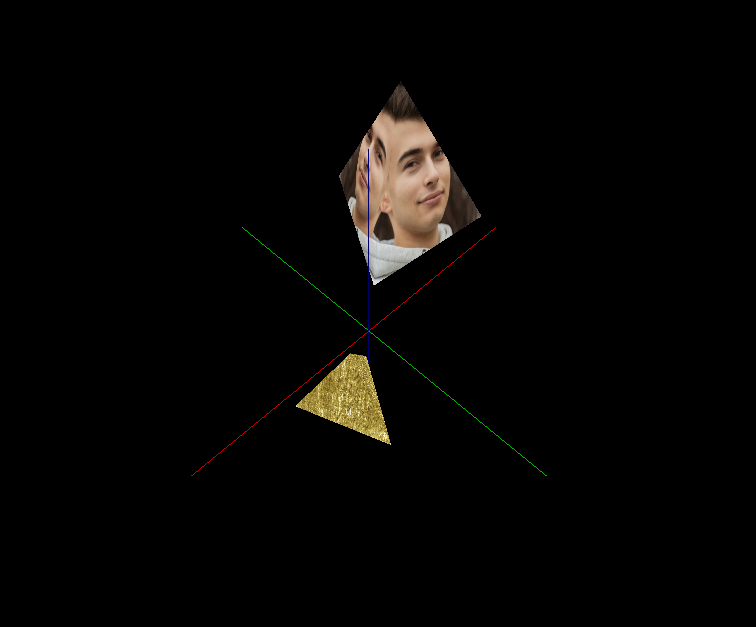
\includegraphics[width=0.8\linewidth, trim={0cm 4cm 0cm 2cm},clip]{img/tex_1.png}
    \caption{Obracające się dwa czworościany z nałożoną teksturą.}
\end{figure}


Dla modelu jajka punkty odwzorowania tekstury zostały przypisane zgodnie z naniesieniem ich na dziedzinę parametryczną równania opisującego model. Wykorzystano stworzony już wcześniej widok, w którym wyświetlane było jajko z przemieszczającymi się źródłami światła.

\begin{figure}[H]
    \centering
    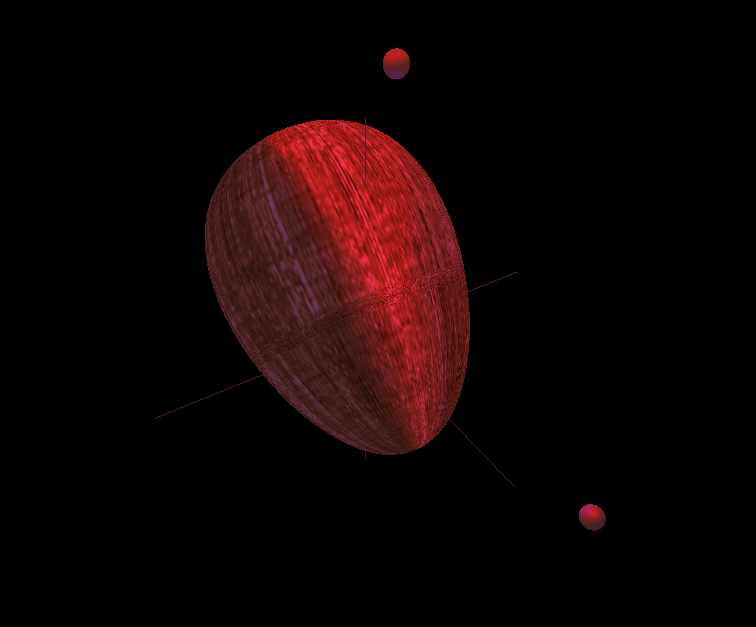
\includegraphics[width=0.8\linewidth, trim={0cm 2cm 0cm 1cm},clip]{img/tex_2.png}
    \caption{Obracający się model jajka z nałożoną teksturą i źródłami światła.}
\end{figure}

